\section{Prompts}
\label{sec:supp-prompts}
All prompts are shown for the viewpoint question of \cref{fig:teaser}; the other tasks differ only in the task-specific sentence, listed after. Images are passed before the text.

\paragraph{direct} (one image: the original)
\begingroup\footnotesize\begin{verbatim}
The image shows a scene.

Imagine you walk a quarter of the way around the scene to your right, keeping
your eyes on the center of the scene. From that new viewpoint, is the orange
cylinder to the left or to the right of the red sphere?
Options: left / right

Reply with only a single line of the form 'Answer: <option>'.
\end{verbatim}
\endgroup
\paragraph{oracle, wrong, shuffled, recon} (two images: the original, then the imagined state). The wording is identical across these four conditions.
\begingroup\footnotesize\begin{verbatim}
The first image shows the current scene. The second image shows the scene from
the new viewpoint described in the question.

Imagine you walk a quarter of the way around the scene to your right, keeping
your eyes on the center of the scene. From that new viewpoint, is the orange
cylinder to the left or to the right of the red sphere?
Options: left / right

Reply with only a single line of the form 'Answer: <option>'.
\end{verbatim}
\endgroup
\paragraph{oracle alone} (one image: the imagined state) The first line of \emph{direct} becomes:
\begingroup\footnotesize\begin{verbatim}
The image shows the scene from the new viewpoint described in the question.
\end{verbatim}
\endgroup
\noindent and analogously for the other tasks (``The image shows the scene after\ldots'').

\paragraph{cot} The last line of \emph{direct} is replaced by a task-specific instruction followed by \texttt{End your reply with a final line of the form 'Answer: <option>'.} The instructions are:
\begingroup\footnotesize\begin{verbatim}
viewpoint: First describe, step by step, how the scene would look from the new
viewpoint, then answer.
swap: First describe, step by step, where every object would be after the
swap, then answer.
stability: First reason, step by step, about where the weight of the upper
blocks rests and what would happen after release, then answer.
\end{verbatim}
\endgroup
\paragraph{Second-image sentence for the other tasks.}
\begingroup\footnotesize
\begin{verbatim}
swap:      The second image shows the scene after the two objects have
           traded places.
stability: The second image shows the scene after the stack was released
           and everything came to rest.
\end{verbatim}
\endgroup
\paragraph{Reconstruction (recon, first stage).} Viewpoint and rearrangement:
\begingroup\footnotesize\begin{verbatim}
List every object in the image. For each one give its name as '<color>
<shape>' (shape is one of: cube, sphere, cylinder) and where it stands on the
floor, seen from above, in meters: x runs from left (negative) to right
(positive) as seen in the image, and z runs from far away (negative) to close
to the camera (positive). All objects are within about 2.5 m of the center of
the scene. Reply with only a JSON list, for example [{"name": "red cube", "x":
0.5, "z": -1.0}, {"name": "blue sphere", "x": -1.2, "z": 0.8}]
\end{verbatim}
\endgroup
Physical outcome:
\begingroup\footnotesize\begin{verbatim}
Look at the stack of flat blocks (ignore any objects lying apart from the
stack). List the blocks from the bottom of the stack to the top. For each give
its color, its width in meters (blocks are 0.9 to 1.5 m wide), and the
horizontal position of its center in meters, from left (negative) to right
(positive) as seen in the image. Reply with only a JSON list, for example
[{"color": "red", "width": 1.2, "x": 0.0}, {"color": "blue", "width": 1.0,
"x": 0.3}]
\end{verbatim}
\endgroup
When a reconstruction leaves out one of the two swapped objects, no imagined state can be rendered and the question is answered from the original image only. This happens on rearrangement for 18 (Qwen3-VL-8B), 3 (Qwen2.5-VL-7B) and 11 (InternVL3-8B) of 200 questions, and never on the other tasks.

Answers are parsed from the last \texttt{Answer:} line, falling back to the last option mentioned anywhere in the reply. Decoding is greedy; the answer limit is 48 new tokens. For \emph{cot} it is 1{,}024; answers that reached it were regenerated with 2{,}048, which under greedy decoding is equivalent to a 2{,}048 limit throughout. For Qwen3-VL-8B, 35 of the first 300 \emph{cot} answers reached 1{,}024 tokens; regenerating them left the number of correct answers unchanged (11), and 14 of them reached 2{,}048 as well, mostly by repeating themselves.

\paragraph{Use of language models.} Besides the VLMs under study, an LLM-based coding assistant was used to help implement the scene generator, renderer and evaluation code, to run and monitor experiments, and to draft and edit text. The authors checked the code, the results and every number and citation in the paper.

\section{Dataset details}
\label{sec:supp-data}
\begin{table}[h]
\centering\small
\begin{tabular}{lccc}
\toprule
 & Viewpoint & Rearrangement & Physical outcome \\
\midrule
Questions & 200 & 200 & 200 \\
Objects per scene & 4--6 (mean 5.0) & 5--6 (mean 5.5) & 3--4 blocks + 1--2 others \\
Options & 2 & 3--4 & 2 \\
Answer balance & 100 left / 100 right & -- & 100 stand / 100 fall \\
Other & \multicolumn{3}{l}{\footnotesize moves: 91 right, 75 left, 34 opposite; 100 flip the current-view answer} \\
\bottomrule
\end{tabular}
\end{table}
\noindent Rearrangement: nearest/second-nearest distance ratio at least 1.4 (median 1.6). Physical outcome: 133 three-block and 67 four-block stacks; unstable stacks fail at the base (69) or at the second block (31). The misleading state is another viewpoint with the opposite answer (viewpoint), a swap with a different partner and a different answer (rearrangement), or the opposite outcome (physical outcome; for stable stacks, the top block falls toward its overhang). Rearrangement answers are skewed toward cylinders (41\% of answers but 33\% of options), so a guesser that prefers cylinders would score about 35\% rather than 29\%.

\section{Additional results}
\label{sec:supp-results}

\paragraph{Egocentric bias by model.} Viewpoint accuracy (\%) on questions whose answer is the \emph{same} from the current view and from the new one, and on those where it \emph{flips}. All models answer from the current view when given only the original image; the imagined view alone resolves this for the 7--8B models, and adding the original image back brings much of the bias back.
\begin{center}\small\begin{tabular}{lcccccc}
\toprule
 & \multicolumn{2}{c}{Img.} & \multicolumn{2}{c}{Img.\ + oracle} & \multicolumn{2}{c}{Oracle only} \\
\cmidrule(lr){2-3}\cmidrule(lr){4-5}\cmidrule(lr){6-7}
Model & same & flip & same & flip & same & flip \\
\midrule
Qwen3-VL-8B & 78.0 & 19.0 & 96.0 & 61.0 & 96.0 & 90.0 \\
Qwen2.5-VL-7B & 93.0 & 3.0 & 99.0 & 53.0 & 97.0 & 98.0 \\
InternVL3-8B & 99.0 & 3.0 & 95.0 & 29.0 & 98.0 & 97.0 \\
Qwen2.5-VL-3B & 54.0 & 41.0 & 60.0 & 51.0 & 50.0 & 55.0 \\
\bottomrule
\end{tabular}
\end{center}

\paragraph{Prompt robustness.} Qwen3-VL-8B on the first 50 questions per task, with the original prompt and with a paraphrase that rewords every instruction and lists the options in reverse order. Individual answers change, most on rearrangement. Under both wordings the oracle helps on all three tasks, and the misleading state hurts on viewpoint and physical outcome but not on rearrangement. The image-only baseline on physical outcome also moves (68 to 52), so at $n=50$ these are coarse checks.
\begin{center}\small\begin{tabular}{lcccccc}
\toprule
 & \multicolumn{2}{c}{View} & \multicolumn{2}{c}{Swap} & \multicolumn{2}{c}{Stab.} \\
\cmidrule(lr){2-3}\cmidrule(lr){4-5}\cmidrule(lr){6-7}
Second input & orig. & para. & orig. & para. & orig. & para. \\
\midrule
Img. & 52.0 & 58.0 & 24.0 & 20.0 & 68.0 & 52.0 \\
Oracle & 66.0 & 70.0 & 42.0 & 50.0 & 96.0 & 88.0 \\
Misl. & 22.0 & 28.0 & 32.0 & 32.0 & 20.0 & 38.0 \\
\bottomrule
\end{tabular}
\end{center}

\paragraph{Stability controls.} In the main runs, the oracle for stable stacks and the misleading image for falling stacks are copies of the original. We therefore re-render both second images from a camera turned by 20$^\circ$ around the stack (same scenes, same prompt), so that no second image equals the original. Accuracy (\%) on stable (``stands'') and falling (``falls'') stacks, 100 each:
\begin{center}\small\begin{tabular}{llcccccc}
\toprule
 & & \multicolumn{3}{c}{Oracle} & \multicolumn{3}{c}{Misl.} \\
\cmidrule(lr){3-5}\cmidrule(lr){6-8}
Model & Camera & stands & falls & all & stands & falls & all \\
\midrule
Qwen3-VL-8B & same & 100.0 & 86.0 & 93.0 & 39.0 & 0.0 & 19.5 \\
 & turned & 90.0 & 81.0 & 85.5 & 28.0 & 22.0 & 25.0 \\
Qwen2.5-VL-7B & same & 100.0 & 60.0 & 80.0 & 85.0 & 0.0 & 42.5 \\
 & turned & 100.0 & 48.0 & 74.0 & 55.0 & 0.0 & 27.5 \\
InternVL3-8B & same & 17.0 & 100.0 & 58.5 & 0.0 & 100.0 & 50.0 \\
 & turned & 5.0 & 100.0 & 52.5 & 0.0 & 100.0 & 50.0 \\
\bottomrule
\end{tabular}
\end{center}
A model that only checked whether the picture changed would answer ``falls over'' for every turned image; the Qwen models do not. As a second check, Qwen3-VL-8B's own reconstructions that show a standing stack (189 of 200) differ from the original in about 6\% of the pixels (range 2.0--11.9\%; a pixel counts as changed when a channel differs by more than 30/255), against about 9\% for the fallen-block oracles (range 6.5--12.3\%). Qwen3-VL-8B says ``stays standing'' for 97.4\% of these reconstructions, and for 94.9\% of the 59 that change as much as some fallen-block oracle; in that shared range, the fallen-block oracles get ``falls over'' 85.9\% of the time. The same amount of change thus leads to opposite answers, depending on what the image shows.

\paragraph{Text traces.} The rearrangement count in \cref{sec:results} is a keyword match on Qwen3-VL-8B's replies: a trace counts when it refers to the swap partner's original position (\eg ``where the green sphere was'', ``the original position of the green sphere''); 198 of 200 do.

\medskip\noindent\begin{minipage}{\linewidth}
\paragraph{A smaller model.} Qwen2.5-VL-3B (bf16) stays near chance in every condition, including the imagined state alone, so it cannot benefit from imagination.
\begin{center}\small\begin{tabular}{lcccccc}
\toprule
Task & Img. & Own & Oracle & Oracle only & Unrel. & Misl. \\
\midrule
View & 47.5 & 49.0 & 55.5 & 52.5 & 51.0 & 43.0 \\
Swap & 32.0 & 33.0 & 39.0 & 42.0 & 36.5 & 36.5 \\
Stab. & 50.0 & 49.0 & 51.0 & 49.5 & 50.0 & 50.0 \\
\bottomrule
\end{tabular}
\end{center}
\end{minipage}

\paragraph{Rescaled reconstructions.} Rescaling Qwen3-VL-8B's reconstructed layout about its centroid so that it spans the scene (no model calls; same replies) changes accuracy from 52.0 to 54.0 on viewpoint and from 36.0 to 41.5 on rearrangement, and the share of reconstructions that imply the correct viewpoint answer from 64.5\% to 65.6\%: the errors are in the relative layout, not the overall scale.

\paragraph{Significance tests.} Exact McNemar tests on the questions both conditions share, Holm-corrected over all rows ($^*$: $p_{\mathrm{Holm}}<0.05$). A and B are the accuracies of the first and second condition named.
{\small\begin{longtable}{llllrrrr}
\toprule
Comparison (A vs.\ B) & Model & Task & & $n$ & A & B & $p_{\mathrm{Holm}}$ \\
\midrule
\endhead
Oracle $>$ Img. & Qwen3-VL-8B & viewpoint & & 200 & 48.5 & 78.5 & $<$0.001$^*$ \\
Misl. $<$ Img. & Qwen3-VL-8B & viewpoint & & 200 & 48.5 & 19.5 & $<$0.001$^*$ \\
Oracle $>$ Unrel. & Qwen3-VL-8B & viewpoint & & 200 & 50.0 & 78.5 & $<$0.001$^*$ \\
Text vs.\ Img. & Qwen3-VL-8B & viewpoint & & 100 & 46.0 & 61.0 & 0.716 \\
Text vs.\ Oracle & Qwen3-VL-8B & viewpoint & & 100 & 61.0 & 72.0 & 1.000 \\
Own vs.\ Img. & Qwen3-VL-8B & viewpoint & & 200 & 48.5 & 52.0 & 1.000 \\
Oracle $>$ Img. & Qwen3-VL-8B & swap & & 200 & 31.0 & 51.5 & $<$0.001$^*$ \\
Misl. $<$ Img. & Qwen3-VL-8B & swap & & 200 & 31.0 & 35.5 & 1.000 \\
Oracle $>$ Unrel. & Qwen3-VL-8B & swap & & 200 & 34.5 & 51.5 & $<$0.001$^*$ \\
Text vs.\ Img. & Qwen3-VL-8B & swap & & 200 & 31.0 & 61.5 & $<$0.001$^*$ \\
Text vs.\ Oracle & Qwen3-VL-8B & swap & & 200 & 61.5 & 51.5 & 0.606 \\
Own vs.\ Img. & Qwen3-VL-8B & swap & & 200 & 31.0 & 36.0 & 1.000 \\
Oracle $>$ Img. & Qwen3-VL-8B & stability & & 200 & 65.5 & 93.0 & $<$0.001$^*$ \\
Misl. $<$ Img. & Qwen3-VL-8B & stability & & 200 & 65.5 & 19.5 & $<$0.001$^*$ \\
Oracle $>$ Unrel. & Qwen3-VL-8B & stability & & 200 & 54.0 & 93.0 & $<$0.001$^*$ \\
Text vs.\ Img. & Qwen3-VL-8B & stability & & 100 & 68.0 & 52.0 & 0.464 \\
Text vs.\ Oracle & Qwen3-VL-8B & stability & & 100 & 52.0 & 95.0 & $<$0.001$^*$ \\
Own vs.\ Img. & Qwen3-VL-8B & stability & & 200 & 65.5 & 55.0 & 1.000 \\
Imagined only $>$ both (flip) & Qwen3-VL-8B & viewpoint & & 100 & 61.0 & 90.0 & $<$0.001$^*$ \\
Oracle@1\,m $>$ Img. & Qwen3-VL-8B & viewpoint & & 200 & 48.5 & 70.0 & $<$0.001$^*$ \\
Oracle@1\,m $>$ Own & Qwen3-VL-8B & viewpoint & & 200 & 52.0 & 70.0 & $<$0.001$^*$ \\
Oracle $>$ Img. & Qwen2.5-VL-7B & viewpoint & & 200 & 48.0 & 76.0 & $<$0.001$^*$ \\
Misl. $<$ Img. & Qwen2.5-VL-7B & viewpoint & & 200 & 48.0 & 24.5 & $<$0.001$^*$ \\
Oracle $>$ Unrel. & Qwen2.5-VL-7B & viewpoint & & 200 & 49.5 & 76.0 & $<$0.001$^*$ \\
Text vs.\ Img. & Qwen2.5-VL-7B & viewpoint & & 200 & 48.0 & 56.0 & 0.821 \\
Text vs.\ Oracle & Qwen2.5-VL-7B & viewpoint & & 200 & 56.0 & 76.0 & $<$0.001$^*$ \\
Own vs.\ Img. & Qwen2.5-VL-7B & viewpoint & & 200 & 48.0 & 52.5 & 1.000 \\
Oracle $>$ Img. & Qwen2.5-VL-7B & swap & & 200 & 32.5 & 51.5 & $<$0.001$^*$ \\
Misl. $<$ Img. & Qwen2.5-VL-7B & swap & & 200 & 32.5 & 34.5 & 1.000 \\
Oracle $>$ Unrel. & Qwen2.5-VL-7B & swap & & 200 & 28.0 & 51.5 & $<$0.001$^*$ \\
Text vs.\ Img. & Qwen2.5-VL-7B & swap & & 200 & 32.5 & 38.0 & 1.000 \\
Text vs.\ Oracle & Qwen2.5-VL-7B & swap & & 200 & 38.0 & 51.5 & 0.092 \\
Own vs.\ Img. & Qwen2.5-VL-7B & swap & & 200 & 32.5 & 37.0 & 1.000 \\
Oracle $>$ Img. & Qwen2.5-VL-7B & stability & & 200 & 50.0 & 80.0 & $<$0.001$^*$ \\
Misl. $<$ Img. & Qwen2.5-VL-7B & stability & & 200 & 50.0 & 42.5 & 1.000 \\
Oracle $>$ Unrel. & Qwen2.5-VL-7B & stability & & 200 & 49.5 & 80.0 & $<$0.001$^*$ \\
Text vs.\ Img. & Qwen2.5-VL-7B & stability & & 200 & 50.0 & 46.5 & 1.000 \\
Text vs.\ Oracle & Qwen2.5-VL-7B & stability & & 200 & 46.5 & 80.0 & $<$0.001$^*$ \\
Own vs.\ Img. & Qwen2.5-VL-7B & stability & & 200 & 50.0 & 46.5 & 1.000 \\
Imagined only $>$ both (flip) & Qwen2.5-VL-7B & viewpoint & & 100 & 53.0 & 98.0 & $<$0.001$^*$ \\
Oracle@1\,m $>$ Img. & Qwen2.5-VL-7B & viewpoint & & 200 & 48.0 & 67.0 & $<$0.001$^*$ \\
Oracle@1\,m $>$ Own & Qwen2.5-VL-7B & viewpoint & & 200 & 52.5 & 67.0 & 0.006$^*$ \\
Oracle $>$ Img. & InternVL3-8B & viewpoint & & 200 & 51.0 & 62.0 & 0.004$^*$ \\
Misl. $<$ Img. & InternVL3-8B & viewpoint & & 200 & 51.0 & 37.0 & $<$0.001$^*$ \\
Oracle $>$ Unrel. & InternVL3-8B & viewpoint & & 200 & 51.0 & 62.0 & 0.006$^*$ \\
Text vs.\ Img. & InternVL3-8B & viewpoint & & 100 & 50.0 & 62.0 & 1.000 \\
Text vs.\ Oracle & InternVL3-8B & viewpoint & & 100 & 62.0 & 56.0 & 1.000 \\
Own vs.\ Img. & InternVL3-8B & viewpoint & & 200 & 51.0 & 48.0 & 1.000 \\
Oracle $>$ Img. & InternVL3-8B & swap & & 200 & 30.5 & 41.5 & 0.038$^*$ \\
Misl. $<$ Img. & InternVL3-8B & swap & & 200 & 30.5 & 34.0 & 1.000 \\
Oracle $>$ Unrel. & InternVL3-8B & swap & & 200 & 35.0 & 41.5 & 1.000 \\
Text vs.\ Img. & InternVL3-8B & swap & & 100 & 34.0 & 36.0 & 1.000 \\
Text vs.\ Oracle & InternVL3-8B & swap & & 100 & 36.0 & 43.0 & 1.000 \\
Own vs.\ Img. & InternVL3-8B & swap & & 200 & 30.5 & 35.0 & 1.000 \\
Oracle $>$ Img. & InternVL3-8B & stability & & 200 & 50.0 & 58.5 & $<$0.001$^*$ \\
Misl. $<$ Img. & InternVL3-8B & stability & & 200 & 50.0 & 50.0 & 1.000 \\
Oracle $>$ Unrel. & InternVL3-8B & stability & & 200 & 50.0 & 58.5 & $<$0.001$^*$ \\
Text vs.\ Img. & InternVL3-8B & stability & & 100 & 50.0 & 62.0 & 1.000 \\
Text vs.\ Oracle & InternVL3-8B & stability & & 100 & 62.0 & 61.0 & 1.000 \\
Own vs.\ Img. & InternVL3-8B & stability & & 200 & 50.0 & 51.0 & 1.000 \\
Imagined only $>$ both (flip) & InternVL3-8B & viewpoint & & 100 & 29.0 & 97.0 & $<$0.001$^*$ \\
\bottomrule
\end{longtable}
}

\clearpage
\section{More examples}
\label{sec:supp-examples}
\begin{center}
  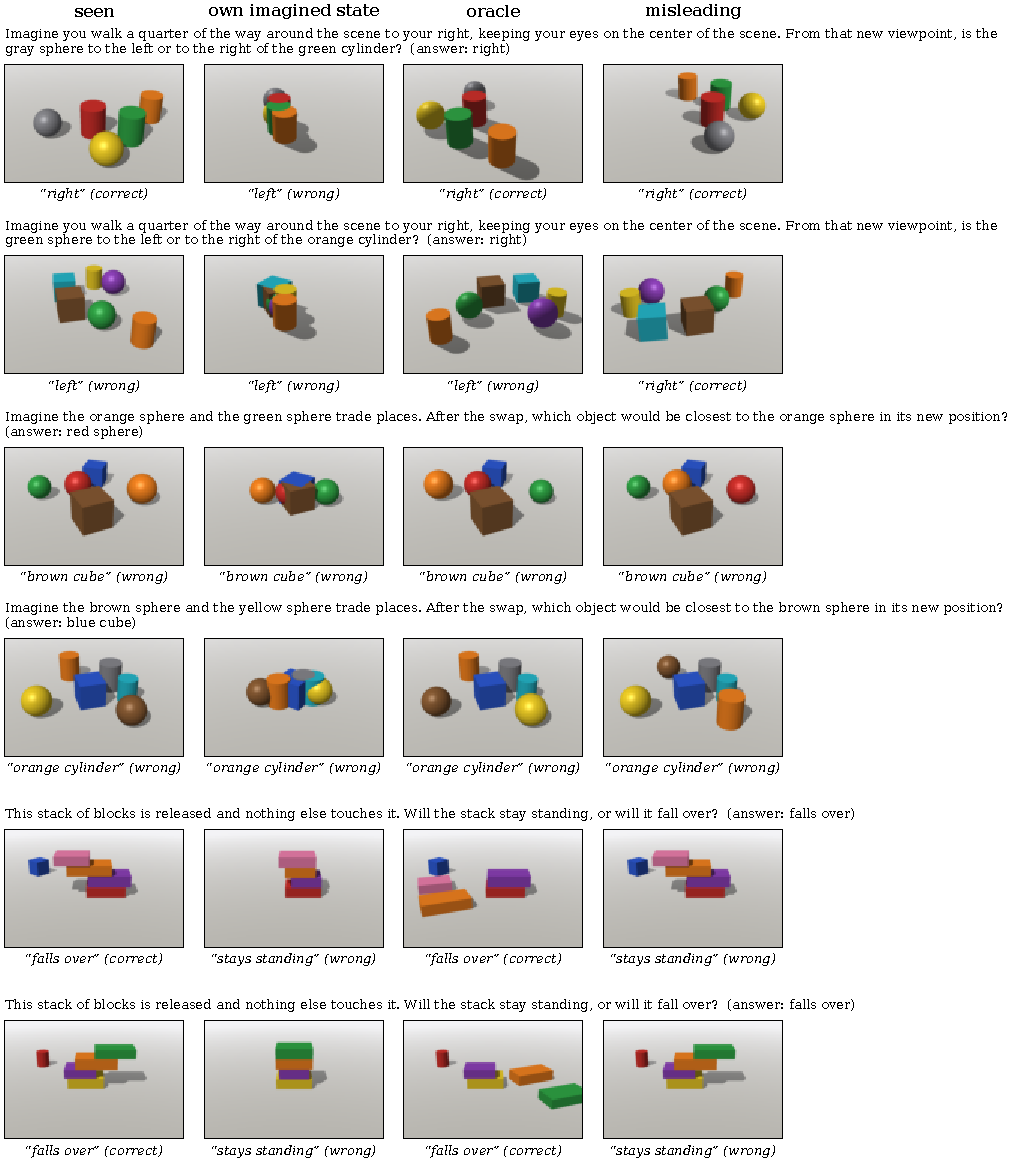
\includegraphics[width=0.86\linewidth]{figs/supp_examples.pdf}
  \captionof{figure}{\textbf{Two questions per task}, with Qwen3-VL-8B's actual answer under each second image (``seen'': the original image only). The examples include failures: on rearrangement the model answers wrongly even with the oracle, and its own reconstructions compress the scene into a cluster (viewpoint) or into a vertical, stable-looking stack (physical outcome).}
  \label{fig:supp-examples}
\end{center}
